\chapter{半空间中的弹性反散射问题的直接成像方法}\label{chap:Elastic}

\section{半空间弹性波方向的 Green 函数}\label{Green Tensor}
\subsection{Neumann Green 函数}\label{Neumann Green Tensor}
设源点$y\in\R^2_+$, 引入半空间弹性波Neumann零边界格林函数$\N(x,y)$, 对任意向量$q\in\R^2$, 其满足如下方程:
\be
& & \Delta_e [\N(x;y)q] + \omega^2 [\N(x,y)q] = -\mathbf{\delta}_y(x) q \ \ \mbox{in }\R^2_+ , \label{eq_n1} \\
& & \sigma(\N(x,y)q)e_2 = 0 \ \ \mbox{on } \Gamma_0, \label{eq_n2}
\ee
其中(\ref{eq_n2})代表该green函数满足半空间自由边界条件,${\delta}_y(x)$代表位于点y的Dirac源。 由于半空间的特性,我们将利用对$x_1$变量作Fourier变换的方式来推导Green函数,令
\be\label{a1}
\hat \N(\xi,x_2;y_2)= \int_\R\N(x_1,x_2;y) e^{-\i (x_1-y_1)\xi} dx_1,\ \ \forall \xi\in\C,
\ee
记 $\G(x,y)$ \cite{ku63} 为弹性波方程的基本解, 且对其$x_1$变量做Fourier变换后有
$\hat{\G}(\xi,x_2;y_2)=\hat{\G}_s(\xi,x_2;y_2)+\hat{\G}_p(\xi,x_2;y_2)$及
\be
& &\hat{\G}_s(\xi,x_2;y_2)=\frac{\i}{2\omega^2}
\left( \begin{array}{cc}
	\mu_s & -\xi\frac{x_2-y_2}{|x_2-y_2|} \\
	-\xi\frac{x_2-y_2}{|x_2-y_2|} & \frac{\xi^2}{\mu_s}
\end{array} \right)e^{\i\mu_s|x_2-y_2|}, \label{G1}\\
& &\hat{\G}_p(\xi,x_2;y_2)=\frac{\i}{2\omega^2} 
\left( \begin{array}{cc}
	\frac{\xi^2}{\mu_p} & \xi\frac{x_2-y_2}{|x_2-y_2|} \\
	\xi\frac{x_2-y_2}{|x_2-y_2|} & \mu_p
\end{array} \right) e^{\i\mu_p|x_2-y_2|}.\label{G2}
\ee
这里$\mu_\alpha=(k_\alpha^2-\xi^2)^{1/2}$且有$\alpha=s,p$, $k_p=\omega/\sqrt{\lam+2\mu}, k_s=\omega/\sqrt{\mu}$为p波和s波的波数。
为了利用基本解$\G(x,y)$的特性,我们令:
\ben
\N_c(x,y)=\N(x,y)-(\G(x,y)-\G(x,y'))
\een
其中$y'=(y_1,-y_2)$ 为y关于$x_1$轴的镜像点。于是由式(\ref{eq_n1}-\ref{eq_n2}),得$\N_c(x,y)$满足如下方程:
\be
& & \Delta_e [\N_c(x;y)q] + \omega^2 [\N_c(x,y)q] = 0 \ \ \mbox{in }\R^2_+ , \label{eq_n3} \\
& & \sigma(\N_c(x,y)q)e_2 =-\sigma(\G(x,y)-\G(x,y')) \ \ \mbox{on } \Gamma_0, \label{eq_n4}
\ee
\begin{remark}
	在全篇论文中,我们假设对于任意的$z\in \mathbb{C}\backslash\{0\}$, $z^{1/2}$是多值函数$\sqrt{z}$ 的如下解析分支:$\Im(z^{1/2})\geq 0$,这对应于在复平面取右半实轴为割支线。则对于$z=z_1+\mathbf{i}z_2$, $z_1,z_2\in\R$,
	\be \label{convention_1}
	z^{1/2}={\rm sgn}(z_2)\sqrt{\frac{|z|+z_1}{2}}+\i\sqrt{\frac{|z|-z_1}{2}},\ \ \forall z\in\C\backslash\bar{\R}_+.
	\ee
	当$z$位于右半实轴的上沿或是下沿时,取$z^{1/2}$为$\ep\rightarrow0^+$ 时$(z+\i\ep)^{1/2}$ 或是 $(z-\i\ep)^{1/2}$的极限即可。
\end{remark}

通过对式(\ref{eq_n3}-\ref{eq_n4})两边作Fourier变换,我们得到关于变量$x_2$的常系数常微分方程组:
\be
 \mu \frac{d^2(e_1^T\hat \N_c q)}{dx_2^2}+\i(\lambda+\mu)\xi\frac{d(e_2^T\hat \N_c q)}{dx_2}+(\omega^2-(\lambda+2\mu)\xi^2)(e_1^T\hat \N_c q) = 0 \label{eq_n5}\\
 (\lambda+2 \mu)\frac{d^2(e_2^T\hat \N_c q)}{dx_2^2}+\i(\lambda+\mu)\xi\frac{d(e_1^T\hat \N_c q)}{dx_2}+(\omega^2-\mu \xi^2)(e_2^T\hat \N_c q) = 0 \label{eq_n6}
\ee
 由于我们需要$\N(x,y)$为外行波解,因此方程 (\ref{eq_n5})的解为如下两个向量:
\ben
 \left[ \begin{array}{cc} \i\mu_s \\ -\i\xi \end{array} \right]e^{\i\mu_s x_2} \ , \ \ \ \ \ \left[ \begin{array}{cc} \i\xi \\ \i\mu_p \end{array} \right]e^{\i\mu_p x_2}
\een
的线性组合。 利用边界条件(\ref{eq_n6})及待定系数法,我们得到:
\be\label{NGT}
\hspace{-2cm}\hat \N_c(\xi,x_2;y_2) =  \frac{\i}{\omega^2\delta(\xi)}\sum_{\alpha,\beta=p,s}\mathbb{A}_{\al\beta}(\xi)e^{\i(\mu_\al x_2+\mu_{\beta} y_2)}, 
\ee
其中 $\varphi(\xi)=k_s^2-2\xi^2$, $\delta(\xi)=\varphi(\xi)^2+4\xi^2\mu_s\mu_p $(Rayleigh方程\cite{achenbach1980}), 以及
\ben
&&{\mathbb{A}_{ss}(\xi)} =
\left( \begin{array}{ll}
	\varphi^2\mu_s & -4\xi^3\mu_s\mu_p \\
	-\xi\varphi^2  & 4\xi^4\mu_p
\end{array} \right),\ \ 
{\mathbb{A}_{sp}(\xi)} =
\left( \begin{array}{ll}
	2\xi^2\varphi\mu_s & -2\xi\varphi\mu_s\mu_p \\
	-2\xi^3\varphi  & 2\xi^2\varphi\mu_p
\end{array} \right),\\
&&
{\mathbb{A}_{ps}(\xi)} =
\left( \begin{array}{ll}
	2\xi^2\varphi\mu_s & 2\xi^3\varphi \\
	2\xi\varphi\mu_s\mu_p  & 2\xi^2\varphi\mu_p
\end{array} \right),\ \ 
{\mathbb{A}_{pp}(\xi)} =
\left( \begin{array}{ll}
	4\xi^4\mu_s & \xi\varphi^2 \\
	4\xi^3\mu_s\mu_p  & \varphi^2\mu_p
\end{array} \right).
\een
按照惯例,原本我们只要对$\hat{\N}(\xi,x_2;y_2)$进行Fourier逆变换就可以得到所需要的Neumann Green函数. 然而,如下面的引理所述, 函数$\delta(\xi)$在实轴上存在零点\cite{achenbach1980, Harris2001Linear},此时我们并不可以对其直接进行Fourier逆变换.
\begin{lem} \label{rayleigh}
	 Rayleigh方程 $\delta(\xi) = 0$在复平面$\C$中有且仅有两个根且记为 $\pm k_R$, 其中$k_R$满足$k_R>k_s$。
\end{lem}

\debproof
 由前文注记中的(\ref{convention_1}), 易得 $\delta(\xi)$ 的割支线为 $C_l=\{\xi=\xi_1+\i\xi_2\in\C: \xi_1\in [-k_s,-k_p],\xi_2=0\}$ 和 
$C_r=\{\xi=\xi_1+\i\xi_2\in\C: \xi_1\in [k_p,k_s],\xi_2=0\}$. 于是$\delta(\xi)$在除 $C_l$ 和 $C_r$ 以外的区域解析。 而在割支线上,$\delta(\xi)$ 可表示成: 
\ben
\delta(\xi)=(k_s^2-2\xi^2)^2+\i\,[4\xi^2(k_s^2-\xi^2)^{1/2}(\xi^2-k_p^2)^{1/2}], \ \ \forall \xi\in C_l\cup C_r.
\een
显然, $\de(\xi)$ 在 $C_l\cup C_r$ 上没有零点。 又因为 $\de(\pm k_s)>0$ , $\de(\pm\infty)<0$ ,由函数的连续性得 $\de(\xi)$ 在区间 $(-\infty,-k_s)\cup(k_s,\infty)$ 上至少存在两个零点, 且由于其对称性,可以记为 $\pm k_R$。 下面, 我们将 $C_l, \ C_r$ 的上下沿分别记为 $C_l^\pm, \ C_r^\pm$。

接下去, 利用幅角原理\cite{Ahlfors1979Complex}可以说明 $\delta(\xi)$ 在整个复平面只存在两个零点。 令 $\Ga_R$ 为半径 $R$ 充分大的圆. 我们考虑 $\mathcal D$ 是被周线 $\Ga_R$, $\Ga_l$ 以及 $\Ga_r$ 包围的区域。 其中 $\Ga_l$ 代表沿着 $C_l^+$ 从 $-k_s$ 到 $-k_p$  及然后沿着 $C_l^-$ 从 $-k_p$ 到 $-k_s$ ; 相应地, $\Ga_r$ 代表 沿着 $C_r^+$ 从 $k_p$ 到 $k_s$ 及然后 沿着 $C_r^-$ 从 $k_s$ 到 $k_p$ 。 因为 $\delta(\xi)$ 在整个整个复平面上没有极点,  我们可以通过幅角原理来计算其在区域
 $\mathcal D$ 中的零点个数 $Z$ :
\be\label{zero}
Z=\frac{1}{2\pi\i}\int_C \frac{\delta'(\xi)}{\delta(\xi)}d\xi.
\ee
由式子(\ref{convention_1})中的定义,我们可以得出当$\xi\in C_r^\pm$时 $\de(\xi)=\de^\pm(\xi)$, 其中
\ben
\de^\pm(\xi)=(k_s^2-2\xi^2)^2\mp\i\,[4\xi^2(k_s^2-\xi^2)^{1/2}(\xi^2-k_p^2)^{1/2}\,]:=f_1(\xi)\mp\i f_2(\xi).
\een
于是可以有如下计算
\ben
\int_{\Ga_r} \frac{\delta'(\xi)}{\delta(\xi)}d\xi&=&\int_{k_p}^{k_s}\left(\frac{{\delta}_{+}' (\xi)}{\delta_{+}(\xi)}-\frac{{\delta}_{-}' (\xi)}{\delta_{-}(\xi)}\right) d\xi\\
&=&2\i\int_{k_p}^{k_s}\frac{f_1'(\xi) f_2(\xi)-f_1(\xi) f_2'(\xi)}{f_1^2(\xi)+ f_2^2(\xi)} d\xi\\
&=&-2\i\arctan \frac{f_2(\xi)}{f_1(\xi)}\Bigg|^{k_s}_{k_p}=0.
\een
相似地, 在 $\xi\in C_r^\pm$ 时也有 $\int_{\Ga_l}\frac{\delta'(\xi)}{\delta(\xi)}d\xi=0$ 。 此外, 当 $|\xi|$ 足够大, 容易得到 $\de(\xi)$ 的渐近形式 $\delta(\xi)=-2(k_s^2-k_p^2)\xi^2+O(1)$ 及  。 于是当 $R\gg 1$ ,可以计算得到
$\int_{\Ga_R} \frac{\delta'(\xi)}{\delta(\xi)}d\xi=4\pi\i$ 。
综上所述, 我们得出 $Z=2$ 。 于是该引理得到证明。
\finproof

为了克服上述问题,我们先假设半空间的介质是耗散的,然后研究其相应的Green函数,最后通过极限吸收原理得到$\N(x,y)$。
记 $\mathbb{N}_{\omega(1+\i\ep)}(x,y)$ 为满足将式子(\ref{eq_n1})中将实圆频率$\omega$ 替换为复圆频率$\om(1+\i\ep)$后相应方程的Green函数。 同样的, 对$\mathbb{N}_{\omega(1+\i\ep)}(x,y)$关于$x_2$变量的Fourier变换,得到$\hat\N_{\omega(1+\i\ep)}(\xi,x_2;y_2)$,且通过相同的推导,其表达式与将(\ref{NGT})中将$k_s, k_p$替换为
$k_s(1+\i\ep), k_p(1+\i\ep)$后相应的式子一致。 下面的两个引理告诉我们,$\hat\N_{\omega(1+\i\ep)}(\xi,x_2;y_2)$的零点所在何处。

\begin{remark}
	通篇全文中, 我们都假设耗散介质所添加的 $\i\ep$ 是足够小的。
\end{remark}
令$\delta_{\om(1+\i\ep)}(\xi)$为将$\delta(\xi)$中的$k_p,k_s$替换成$k_s(1+\i\ep), k_p(1+\i\ep)$后相应的复Rayleigh方程。 为了展现 $\delta_{\om(1+\i\ep)}(\xi)$ 的零点 与 $\delta(\xi)$ 的零点的关系,我们先来刻画在何种情况下可以结合或是分离根式 $z^{1/2}$ 。
\begin{lem}\label{lem23}
	令 $0<\ep<1$ , 假设 $z=R e^{\i\phi}$, $(1+\i\varepsilon)=r e^{\i\psi}$ 其中有 $0\leq\phi<2\pi$, $0<\psi<\pi/2$ 和  $R,r>0$. 于是等式
	\be
	z^{1/2}=(1+\i\varepsilon)(\frac{z}{{1+\i\varepsilon}^2})^{1/2}
	\ee
	当且仅当  $2\psi\leq\phi<2\pi$
\end{lem}
\debproof
令 $z_\ep=z/(1+\i\ep)^2:=R_\ep e^{\i\phi_\ep}$ , 其中 $0\leq\phi_\ep<2\pi$。于是,易得当 $2\psi\leq\phi<2\pi$ 时, 成立 $\phi_\ep=\phi-2\psi , \ R_\ep=R/r$ ,则有
\ben
z^{1/2}=\sqrt{R}e^{\i\phi/2}=\sqrt{R/r}\sqrt{r}e^{\i(\phi/2-\psi)+\i\psi}=\sqrt{R_\ep}\sqrt{r}e^{\i(\phi_\ep)+\i\psi}=(1+\i\ep)z_\ep^{1/2}
\een
同样地, 当 $0\leq\phi<2\psi$ 时, 成立 $\phi_\ep=\phi-2\psi+2\pi$ 则有 $z^{1/2}=-(1+\i\ep)z_\ep^{1/2}$。 引理得证
\finproof

下面的引理告诉我们,$\hat\N_{\omega(1+\i\ep)}(\xi,x_2;y_2)$的零点所在何处。

\begin{lem}\label{complex_rayleigh}
	复Rayleigh方程 $\delta_{\om(1+\i\ep)}(\xi)$在$\C\bks\bar{\Om}$中有且仅有两个根且为$\pm k_R(1+\i\ep)$。 其中集合$\Om$为
	\be\label{set:Om}
	\Omega := \{\xi_1+\i\xi_2 \in \mathbb{C} \ | \ k_p(1+\i\ep)<\xi_1\xi_2<k_s(1+\i\ep) \ , \  \ \xi_2>\xi_1(1+\i\ep)\}
	\ee
\end{lem}
\debproof
 我们定义 $\mu_\ep=(k^2(1+\i\ep)^2-\xi^2)^{1/2},k\in\R^+$ , 令 $\xi=\xi_1+\i\xi_2,\xi_1,\xi_2\in\R$ and $(1+\i\varepsilon)=r e^{\i\psi}$ 。通过简单的计算, 我们有
\be
\mu_\ep^2 = k^2(1-\ep^2)-\xi_1^2+\xi_2^2+\i(2k^2\ep-2\xi_1\xi_2):=Re^{\i\Theta} := a_1+\i a_2
\ee
定义 $\Delta:=\{ \xi | 2\psi\leq\Theta<2\pi \} $ , 于是由引理 \ref{lem23} 成立 $ \mu_\ep = (k^2-\xi_\ep^2)^{1/2} (1+\i\ep)$ 当 $\xi \in\Delta$ ,另一方面 $ \mu_\ep = - (k^2-\xi_\ep^2)^{1/2} (1+\i\ep)$ 当 $\xi \notin\Delta$ 。 由于 $\ep$ 足够小, 我们可以有如下关于集合 $\Delta$ 的等价形式:
\be\nn
\Delta &=& (\pi/2\geq\Theta<2\pi)\cup(2\psi<\Theta<\pi/2) \\
&=& \{ \xi | a_1 \leq 0 \} \cup \{ \xi | a_2 \leq 0 \} \cup \{ \xi | a_1 >0,a_2 >0 \ ,\ \ \tan\Theta \geq \tan(2\psi) \} \\ \nn
&:=& \Delta_1 \cup \Delta_2 \cup \Delta_3
\ee
Our goal now is to show where domain $\Delta$ occupies. A simple computation show that
\be
\Delta_1 = \{ \xi | \xi_1^2-\xi_2^2 \geq k^2(1-\ep^2) \}  \\
\Delta_2 = \{ \xi | \xi_1\xi_2 \geq k^2\ep \}
\ee
and
\be
\hspace{-2cm}
\Delta_3 = \{ \xi | \xi_1^2-\xi_2^2 \leq k^2(1-\ep^2), \xi_1\xi_2 \leq k^2\ep ,
\frac{k^2\ep-\xi_1\xi_2}{k^2(1-\ep^2)-(\xi_1^2-\xi_2^2)} \geq \frac{\ep}{1-\ep^2} \}
\ee
The domains denote by $\Delta_1,\Delta_2$ are obvious in complex plane. To locate $\Delta_3$ in complex plane, we divide $\Delta_3$ into tree parts $\Delta_3=\Delta_{31}\cup\Delta_{32}\cup\Delta_{33}$
where
\ben
\Delta_{31} &=& \{ \xi_1\xi_2 \leq 0, 0\leq\xi_1^2-\xi_2^2 \leq k^2(1-\ep^2) \} \\
\Delta_{32} &=& \{ 0 \leq \xi_1\xi_2 \leq k^2\ep, 0\leq\xi_1^2-\xi_2^2 \leq k^2(1-\ep^2), \frac{\xi_1\xi_2}{\xi_1^2-\xi_2^2} \leq \frac{\ep}{1-\ep^2} \} \\
&=& \{ 0 \leq \xi_1\xi_2 \leq k^2\ep, 0\leq\xi_1^2-\xi_2^2 \leq k^2(1-\ep^2), \frac{\xi_2}{\xi_1} \leq \ep \} \\
\Delta_{33} &=& \{ \xi_1\xi_2 \leq 0, \xi_1^2-\xi_2^2 \leq 0 ,\frac{\xi_1\xi_2}{\xi_1^2-\xi_2^2} \geq \frac{\ep}{1-\ep^2} \} \\
&=& \{ \xi_1\xi_2 \leq 0, \xi_1^2-\xi_2^2 \leq 0 ,-\frac{\xi_1}{\xi_2} \geq \ep \}
\een
Substituting $k_s,k_p$ into $\mu_\ep$ and let $\Delta_s,\Delta_p$ denote their corresponding areas, we have
\be
\C\bks\Omega = (\Delta_s \cap \Delta_p )\cup (\C\backslash(\Delta_s \cup \Delta_p))
\ee
Moreover, when $\xi\in\Omega$ it is easy to see $\delta_\ep(\xi)=\delta(\xi)(1-\i\ep)^4 $.
This complete the proof by lemma \ref{lem2.1}
\finproof

 由引理\ref{complex_rayleigh} 我们发现 $\hat\N_{\omega(1+\i\ep)}(\xi,x_2;y_2)$ 在实轴上没有极点, 可以对其直接进行逆Fourier变换。 于是, Neumann Green函数 $\mathbb{N}(x,y)$ 可以利用极限吸收原理得到,即为
\be\label{NGT1}
\N(x,y)=\lim_{\ep\to 0^+} \N_{\om(1+\i\ep)}(x,y)=\lim_{\ep\to 0^+}\frac{1}{2\pi}\int_\R\hat \N_{\om(1+\i\ep)}(\xi,x_2;y_2) e^{\i(x_1-y_1)\xi} d\xi.
\ee

现在, 我们已经得到 Neumann Green函数的具体表达形式了。 但是,式子(\ref{NGT1})中这种极限形式并不利于我们分析该函数的具体性质,特别是其无穷远处的衰减阶数。 为了便于得到更加简洁的表达形式, 我们引入下面这个关于柯西主值(cf. e.g. \cite[Chapter 4, Theorem 5]{Kuroda})的引理
\begin{lem}\label{cauchy_pv}
	令 $a,b\in\R,\  a<b$, 且 $t_0\in (a,b)$. 如果 $\gamma$ 在$[a,b]$上 H\"older 连续, 即存在常数 $\alpha\in (0,1]$ 及 $C>0$ 对于任意 $s,t\in [a,b]$, $|\gamma(s)-\gamma(t)|\le C|s-t|^\alpha$, 于是有
	\ben
	\lim_{z\to t_0,\pm\Im z>0}\int^b_a\frac{\gamma(t)}{t-z}dt={\rm p.v.}\int^b_a\frac{\gamma(t)}{t-t_0}dt\pm\pi\i\ga(t_0),
	\een
	其中 ${\rm p.v.}\int^b_a$ 表示积分的Cauchy主值。
\end{lem}

通过引理 \ref{rayleigh}, 引理 \ref{complex_rayleigh} , 易知 $\hat\N_{\omega(1+\i\ep)}(\xi\mp k_R(1+\i\ep))$ 在点 $\pm k_R$ 的某个小领域内解析且
关于 $\ep$ 一致有界。 于是, 对于足够小的 $d>0$,  成立:
\be
& &\lim_{\ep\to 0^+}\int_{\pm k_R-d}^{\pm k_R+d}\hat \N_{\om(1+\i\ep)}(\xi,x_2;y_2) e^{\i(x_1-y_1)\xi} d\xi \\
&=& \lim_{\ep\to 0^+}\int_{\pm k_R-d}^{\pm k_R+d}\frac{\hat \N(\xi,x_2;y_2)(\xi-k_R)}{\xi\mp k_R(1+\i\ep)} e^{\i(x_1-y_1)\xi} d\xi
\ee

然后利用引理 \ref{cauchy_pv} , 表达式 (\ref{NGT1}) 及上面的等式, 可以得到如下 Neumann Green 函数的表达式:
\ben
\N(x,y)&=&\frac{1}{2\pi}\,{\rm p.v.}\int_{\R}\hat \N(\xi,x_2;y_2) e^{\i(x_1-y_1)\xi} d\xi\\
& &-\frac{1}{2\omega^2}
\left[\sum_{\alpha,\beta=p,s}\frac{\mathbb{A}_{\al\beta}(\xi)}{\de'(\xi)}e^{\i(\mu_\al x_2+\mu_\beta y_2)+\i(x_1-y_1)\xi}\right]^{k_R}_{-k_R},\ \ \forall x,y\in\R^2_+,
\een
这里 $[f(\xi)]^b_a:=f(b)-f(a)$ 。

\begin{remark}
	值得注意的是, 由于 $\hat\N(\xi,x_2;y_2)$ 在实轴上存在极点及研究目的的区别, 导致最终$\N(x,y)$可以存在多种等价的表达形式。 例如, 在文献 \cite{nedelec2011} 中 Duran 等人是利用 Cauchy 积分定理以及留数定理将积分路径从实轴变换到双曲线上, 从而避开被积函数的极点。 可以证明的是, 本文中推导出的 Green 函数与文献 \cite{nedelec2011} 中的是一致的。 
\end{remark}

观察式子 (\ref{G1}) , (\ref{G2}) , 及 (\ref{NGT}), 通过简单的变量替换, 我们易得 Neumann Green 函数满足如下对称性,即
\be\label{symm}
\N(x,y)=\N(y,x)^T \ \ \ \ \ \ \ \forall x,y\in\R^2_+
\ee
对于 $x_s\in\Ga_0$ 的情况, 我们定义这种 Green 函数 $\N(x,x_s),x\in\R^2_+$ 为 $\N(x,y)$ 在 $y\in\R^2_+,  \  y\to x_s$ 时的极限。
由于半空间反散射问题中的点源一般都位于界面上, 所以接下去我们重点研究 $x\in\Ga_0 ,  \ y\in\R^2_+$ 时的 Neumann Green 函数 $\N(x,y)$ 。
通过 (\ref{G1}) , (\ref{G2}) , (\ref{NGT}), 简单的计算可以简化 $\N(x,y)$ :
\be
\hat
\N(\xi,0;y_2)&=&\frac{\i}{\mu\delta(\xi)} \Bigg[ \Bigg(
\begin{array}{cc}
	2\xi^2\mu_s & -2\xi\mu_s\mu_p\\
	-\xi\varphi & \mu_p\varphi
\end{array} \Bigg)e^{\i\mu_p y_2}
+ \Bigg(
\begin{array}{cc}
	\mu_s\varphi & \xi\varphi \\
	2\xi\mu_s\mu_p & 2\xi^2\mu_p
\end{array} \Bigg)e^{\i\mu_s y_2} \Bigg] \nonumber\\
&:=&\frac{1}{\delta(\xi)}(\Np(\xi)e^{\i\mu_p y_2}+\Ns(\xi)e^{\i\mu_s y_2}), \label{d2}
\ee
且, 当 $x\in\Ga_0, y\in\R^2_+$,
\be\label{c8}
\N(x,y)=\frac{1}{2\pi}\,{\rm p.v.}\int_{\R}\hat \N(\xi,0;y_2) e^{\i(x_1-y_1)\xi} d\xi+\frac\i 2
\left[\sum_{\al=p,s}\frac{\Na(\xi)}{\de'(\xi)}e^{\i\mu_\al y_2+\i(x_1-y_1)\xi)}\right]^{k_R}_{-k_R}.
\ee

为了便于研究 Neumann Green 函数在边界 $\Ga_0$上水平方向的渐近行为, 我们下面引理中更为有用的表达形式。


\begin{lem}\label{lem:2.3} 令 $x\in\Ga_0 \ , y\in \R^2_+$ 以及 $\phi\in (-\pi/2,\pi/2)$ 且存在如下表达 $y_2=|x-y|\cos\phi \ ,
	x_1-y_1=|x-y|\sin\phi$ 。 假设 $x_1\not= y_1$, 于是可以得到
	\be
	\N(x,y)&=&\frac{1}{2\pi}\int_L\mathbb{N}_0(t)\cos(t+\phi)e^{\i\lam\cos t}dt\pm\i
	\left[\sum_{\al=p,s}\frac{\Na(\xi)}{\de'(\xi)}e^{\i\mu_\al y_2+\i(x_1-y_1)\xi}\right]_{\xi=\pm k_R},\label{h3}
	\ee
	其中 $\lam=k_s|x-y|$, $L$ 为复平面中的积分路径即 从 $-\pi/2+\i\infty$ to $-\pi/2$, $-\pi/2$ 到 $\pi/2$, 接着从 $\pi/2$ 到 $\pi/2-\i\infty$  ( 见图例 \ref{figure_trans}), 这里符号 $\pm$ 取决于 ${\rm sgn}(x_1-y_1)=\pm 1$, 且定义表达式:
	\be\label{h2}
	\mathbb{N}_{0}(t)=\sum_{\al=p,s}k_s\,\frac{\Na(k_s\sin(t+\phi))}{\de(k_s(\sin(t+\phi))}.
	\ee
\end{lem}

\debproof
不失一般性, 我们可以假设 $x_1>y_1$, 因此有 ${\rm sgn}(x_1-y_1)=1$。 注意到 $\hat{\N}(\xi,0;y_2)=\sum_{\al=p,s}\frac{\Na(\xi)}{\de(\xi)}e^{\i (y_2\mu_\al+(x_1-y_1)\xi)}$,所以对于 $\al=p,s$, 我们可以做经典的三角变量替换, 即为 $\xi=k_\al\sin t$ 。 由于三角函数的周期性, 这里我们规定 $-\pi<\Re t \leq\pi$ 以保证变换的一一对应。 相应地, $\xi$ 在复平面中的积分路径 $\R$ 对应于 $t$ 所在复平面中的积分路径 $L$ 。 于是得到如下等式:
\ben
& &\frac{1}{2\pi}\,{\rm p.v.}\int_{\R}\hat \N(\xi,0;y_2) e^{\i(x_1-y_1)\xi} d\xi \\
&=&\frac 1{2\pi}\,{\rm p.v.}\int_L\sum_{\al=p,s}k_s\,\frac{\Na(k_s\sin t)}{\de(k_s\sin t)}\cos t\, e^{\i \lam\cos (t-\phi)}dt.
\een
令 $L_{-\phi}$ 为 $L$ 平移 $-\phi$ 后的积分路径, 立即得到
\be\label{h1}
& &\frac{1}{2\pi}\,{\rm p.v.}\int_{\R}\hat \N(\xi,0;y_2) e^{\i(x_1-y_1)\xi} d\xi \\
&=&\frac 1{2\pi}\,{\rm p.v.}\int_{L_{-\phi}}\mathbb{N}_0(t)\cos (t+\phi)\,e^{\i\lam\cos t}dt,
\ee
这里 $\mathbb{N}_0(t)$ 如 (\ref{h1}) 所定义。

设 $t_R\in L$ 满足等式 $k_R=k_s\sin t_R$, 于是 $k_R$ 即为 $t_R$ 在积分变换 $\xi=k_s\sin t$ 下的像点。 特别地, 由于 $k_R>k_s$, 则存在  $s_R>0$ 使得  $t_R=\pi/2-\i s_R\in L$ 。 对于任意$\ep>0$,令 $ L^\ep$ 表示如下积分路径: $-\pi/2+\i\infty\to -\pi/2+\i (s_R+\ep)\cup\pa B^+_\ep(-t_R)\to -\pi/2+\i(s_R-\ep)\to -\pi/2
\to\pi/2\to\pi/2-\i(s_R-\ep)\to\pa B^+_\ep(t_R)\to\pi/2-\i(s_R+\ep)\to\pi/2-\i\infty$, 其中 $\pa B^+_\ep(\pm t_R)$ 表示圆心在 $\pm t_R$ 半径为 $\ep$ 的右半圆  (见图例 \ref{figure_trans})。 然后, 令 $L^\ep_{-\phi}$ 为 $L^\ep$ 平移 $-\phi$ 后的积分路径。 于是, 利用 Cauchy 主值的定义及留数定理, 我们可以得知
\ben
& &\frac 1{2\pi}\,{\rm p.v.}\int_{L_{-\phi}}\mathbb{N}_0(t)\cos(t+\phi)\,e^{\i \lam\cos t}dt \\
&=&\lim_{\ep\to 0^+}\frac 1{2\pi}\int_{L^\ep_{-\phi}}\mathbb{N}_0(t)\cos (t+\phi)\,e^{\i \lam\cos t}dt\\
& &+\frac\i 2\sum_{t'=\pm t_R}{\rm Res}(\mathbb{N}_0(t)\cos (t+\phi)e^{\i \lam\cos t},t').
\een
\begin{figure}[htbp]
	\centering
	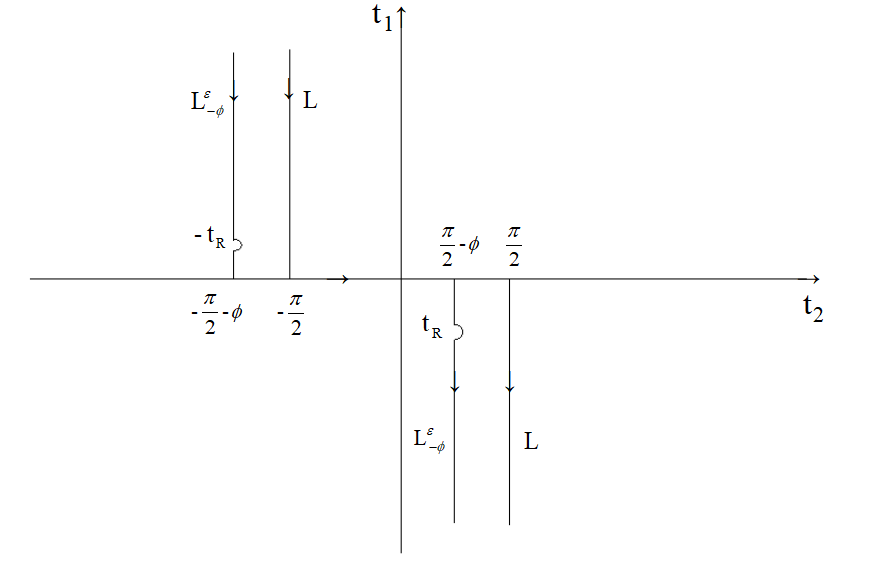
\includegraphics[width=\textwidth]{./Img/graphic/transformation4.png}
	\caption{ 积分路径 $L$ 和 $L^\ep_{-\phi}$}\label{figure_trans}
\end{figure}
通过简单的计算, 易得相应留数为:
\ben
& &\frac\i 2\sum_{t'=\pm t_R}{\rm Res}(\mathbb{N}_0(t)\cos (t+\phi)e^{\i \lam\cos t},t')\\
&=&\frac \i 2\sum_{\xi=\pm k_R}\sum_{\al=p,s}\frac{\Na(\xi)}{\de'(\xi)}e^{\i (y_2\mu_\al+(x_1-y_1)\xi)}.
\een
另一方面,通过 Cauchy 积分定理, 我们得到 
\ben
\frac 1{2\pi}\int_{L^\ep_{-\phi}}\mathbb{N}_0(t)\cos (t+\phi)\,e^{\i \lam\cos t}dt
=\frac 1{2\pi}\int_{L}\mathbb{N}_0(t)\cos (t+\phi)\,e^{\i \lam\cos t}dt.
\een
最后利用 (\ref{c8}) 和 (\ref{h1}) 引理得证。
\finproof
 
 上述引理是我们研究 Neumann Green 函数 $\N(x,y)$ 在界面 $\Ga_0$ 上当 $x\to\infty$ 时衰减行为估计的一个出发点。 下面, 我们先回顾下关于振荡积分衰减阶数估计的 Van der Corput 引理 \cite[P.152]{grafakos} 。
 
 \begin{lem}\label{van}
 	令 $\lam\ge 1$, $f\in C[a,b]$且其导函数绝对可积, 如果 $u\in C^k[a,b]$, 其中 $k\ge 1$ 及 $a<b$, 我们就有如下结论 \\
 	{\rm 1}. 如果 $|u'(t)|\ge 1$ 对于任意 $t\in (a,b)$ 成立,且 $u'$ 在 $(a,b)$ 上单调, 就断言
 	\ben
 	\left|\int^b_a f(t)e^{\i\lambda u(t)}dt\right|\le
 	3\lambda^{-1}\left(|f(b)|+\int^b_a |f'(t)|dt\right).
 	\een
 	{\rm 2}. 对于 $k\geq2$ 时, 如果 $|u^{(k)}(t)|\ge 1$ 对于任意 $t\in (a,b)$ 成立, 就断言 
 	\ben
 	\left|\int^b_a f(t)e^{\i\lambda u(t)}dt\right|\le
 	12k\lambda^{-1/k}\left(|f(b)|+\int^b_a|f'(t)|dt\right).
 	\een
 \end{lem}

在文献\cite{RTMhalf_aco}中,Chen 等对半空间逆时偏移算法的研究时,引理 \ref{van} 起到了关键的作用。该引理相对于驻相定理的优势在于,对于振幅函数 $f(t)$ 的光滑性要求更低,且对于 $\lambda$ 阶数的刻画具有一致性。然而, 当振幅函数具有弱奇异点时,直接使用引理 \ref{van} 就行不通了。 幸运的是,经过研究我们发现 当振幅函数存在弱奇异点, 且其与相位函数 $\phi(t)$ 的驻相点的距离存在正下界时, Van der corput 引理仍然成立,如下述引理刻画。


\begin{lem}\label{lem:2.5}
	令 $\lam\ge 1$, 假设$f\in C[-\pi/2,\pi/2]$ 且其导函数绝对可积。 于是对任意区间 $(a,b)\subset (-\pi/2,\pi/2)$, 可以得到
	\be\label{c1}
	\left|\int_a^bf(t)e^{\i\lam\cos t}dt\right| 
	\leq C\lam^{-1/2}\left(|f(0)|+\int_a^b|f'(t)|dt\right),
	\ee
	这里常数 $C$ 与 $a,b,\lam$ 及被积函数 $f$ 无关。 
	此外, 令 $\kappa\in (0,1)$ 以及 $\phi\in (-\pi/2,\pi/2)$ 满足条件 $|\phi|\geq\phi^*>\arcsin \kappa:=\phi_\kappa$ , 可以得到
	\be\label{c3}
	\left|\int_{-\frac\pi 2}^{\frac\pi 2}f(t)(\kappa^2-\sin^2(t+\phi))^{-1/2}e^{\i\lam\cos t}dt\right| 
	\leq C\lam^{-1/2}\left(|f(0)|+\int_{-\frac\pi 2}^{\frac \pi2}|f'(t)|dt\right),
	\ee
	这里常数 $C$ 只与 $\phi^*$ 和 $\kappa$ 有关。
\end{lem}
\debproof
The estimate (\ref{c1}) follows directly from Lemma \ref{van} since the interval $(a,b)$ can be divided into several subintervals so that in each subinterval, either $|\sin t|$ or $|\cos t|$ is bounded below by $1/\sqrt 2$. 

Let $g(t)=\kappa^2-\sin^2(t+\phi)$. It is easy to see that $g(t)$ has two zeros $t_1, t_2$ in $(-\pi/2,\pi/2]$, where
$t_1=\phi_\kappa-\phi$ and $t_2=-\phi_\kappa-\phi$ or $t_2=\pi-\phi_\kappa-\phi$ depending on whether $\phi+\phi_\kappa<\pi/2$ or $\phi+\phi_\kappa\ge \pi/2$. Without loss of generality, we assume the later case and thus $t_2=\pi-\phi_\kappa-\phi$. 

Let $\ep_0=\min(\frac{\phi^*-\phi_\kappa}{2},\frac{\phi_\kappa}{2})>0$. Obviously, $t_1-\ep_0\le -\pi/2, t_1+\ep_0\le -(\phi^*-\phi_\kappa)/2$ and $t_2-\ep_0\ge(\phi^*-\phi_\kappa)/2$. We divide $(-\pi/2,\pi/2)$ into five intervals:
$I_1=(-\pi/2,t_1-\ep_0), I_2=(t_1-\ep_0,t_1+\ep_0), I_3=(t_1+\ep_0,t_2-\ep_0), I_4=(t_2-\ep_0,t_2+\min(t_2+\ep_0,\pi/2))$ and $I_5=(\min(t_2+\ep_0,\pi/2),\pi/2)$.
By (\ref{c1}) we have
\be\label{c4}
\hspace{-2.5cm}  \left|\int_{I_1\cup I_3\cup I_5}f(t)(\kappa^2-\sin^2(t+\phi))^{-1/2}e^{\i\lam\cos t}dt\right| 
\leq C\lam^{-1/2}\left(|f(0)|+\int_{-\frac\pi 2}^{\frac\pi 2}|f'(t)|dt\right),
\ee
where the constant $C$ depends only on $\phi^*$ and $\kappa$. 

Now we estimate the integral in $I_2, I_4$.  We first observe that $|\sin t|\ge \sin((\phi^*-\phi_\kappa)/2)$ in $I_2\cup I_4$. Moreover, $|g'(t)|=|\sin(2(t+\phi))|\ge \min(\sin\phi_\kappa,\sin(\phi^*+\phi_\kappa))$ in $I_2\cup I_4$. Let $\de\in (0,\ep_0)$ be sufficiently small. Since $g(t_j)=0, j=1,2$, by the mean value theorem, we have
\ben
\hspace{-1cm}|g(t)|\ge \min(\sin\phi_\kappa,\sin(\phi^*+\phi_\kappa))\de,\ \ \forall \de\le |t-t_j|\le \ep_0,j=1,2.
\een
By integration by parts we then obtain
\ben
\hskip-1cm& &\left|\int_{t_1-\ep_0}^{t_1-\de}f(t)g(t)^{-1/2}e^{\i\lam\cos t}dt\right| \le C\delta^{-1/2}\lam^{-1}\left(|f(0)|+\int_{-\frac\pi 2}^{\frac \pi 2}|f'(t)|dt\right).
\een
Similarly, 
\ben
\hspace{-1.cm}\left|\int_{t_1+\de}^{t_1+\ep_0}f(t)g(t)^{-1/2}e^{\i\lam\cos t}dt\right| 
\le C\delta^{-1/2}\lam^{-1}\left(|f(0)|+\int_{-\frac\pi 2}^{\frac \pi 2}|f'(t)|dt\right).
\een
Finally, 
\ben
\hspace{-1.cm}\left|\int_{t_1-\delta}^{t_1+\de}f(t)g(t)^{-1/2}e^{\i\lam\cos t}dt\right| 
&\leq&C\max_{t\in(-\pi/2,\pi/2)}|f(t)|\int_{-\delta}^{\de}|\kappa -\sin(\phi_\kappa+t)|^{-1/2}dt\\
\hspace{-1.cm}&\leq&C\de^{1/2}\max_{t\in(-\pi/2,\pi/2)}|f(t)|.
\een
In conclusion, by taking $\delta=\lam^{-1}$, we obtain
\ben
\hspace{-1.5cm}\left|\int_{I_2}f(t)(\kappa^2-\sin^2(t+\phi))^{-1/2}e^{\i\lam\cos t}dt\right| 
\leq C\lam^{-1/2}\left(|f(0)|+\int_{-\frac\pi 2}^{\frac \pi 2}|f'(t)|dt\right).
\een
The integral in $I_4$ can be estimated similarly. This completes the proof by combining with the estimate in (\ref{c4}).
\finproof

\subsection{Dirichlet Green 函数}\label{Dirichlet Green Tensor}


\section{正散射问题的适定性}

